\documentclass[12pt, a4paper]{article}

% --- UNIVERSAL PREAMBLE BLOCK ---
\usepackage[a4paper, top=2.5cm, bottom=2.5cm, left=2cm, right=2cm]{geometry}
\usepackage{fontspec}

\usepackage[vietnamese, bidi=basic, provide=*]{babel}

\babelprovide[import, onchar=ids fonts]{vietnamese}
\babelprovide[import, onchar=ids fonts]{english}

% Set default/Latin font to Sans Serif in the main (rm) slot
\babelfont{rm}{Noto Sans}
\babelfont[vietnamese]{rm}{Noto Sans}

\usepackage{enumitem}
\setlist[itemize]{label=-}
% --------------------------------

\usepackage{amsmath, amssymb, amsfonts}
\usepackage{graphicx}
\usepackage{algorithm}
\usepackage{algpseudocode}
\usepackage{booktabs}
\usepackage{hyperref}
\usepackage{listings}
\usepackage{xcolor}

% Cấu hình hiển thị Code Python
\definecolor{codegreen}{rgb}{0,0.6,0}
\definecolor{codegray}{rgb}{0.5,0.5,0.5}
\definecolor{codepurple}{rgb}{0.58,0,0.82}
\definecolor{backcolour}{rgb}{0.95,0.95,0.92}
\lstdefinestyle{mystyle}{
    backgroundcolor=\color{backcolour},   
    commentstyle=\color{codegreen},
    keywordstyle=\color{magenta},
    numberstyle=\tiny\color{codegray},
    stringstyle=\color{codepurple},
    basicstyle=\ttfamily\footnotesize,
    breakatwhitespace=false,         
    breaklines=true,                 
    captionpos=b,                    
    keepspaces=true,                 
    numbers=left,                    
    numbersep=5pt,                  
    showspaces=false,                
    showstringspaces=false,
    showtabs=false,                  
    tabsize=4
}
\lstset{style=mystyle}

\title{\textbf{NGHIÊN CỨU TỐI ƯU HÓA NĂNG LƯỢNG TRONG QUY HOẠCH ĐƯỜNG ĐI 2.5D VÀ ĐIỀU KHIỂN DỰ BÁO PHI TUYẾN (NMPC) DỰA TRÊN MÔ HÌNH VẬT LÝ}}
\author{Nhóm 3}
\date{Ngày 14 tháng 4, 2026}

\begin{document}

\maketitle

\begin{abstract}
Nghiên cứu này (thuộc khuôn khổ nhiệm vụ Động lực học \& Điều khiển) trình bày việc tích hợp các mô hình vật lý bao gồm cơ học đất (Bekker-Wong) và tiêu hao năng lượng động lực học (Minetti) vào các thuật toán quy hoạch đường đi trên địa hình 2.5D. Bài báo tiến hành thực nghiệm, tập trung phân tích sâu hiệu năng của thuật toán tìm kiếm trên lưới (Weighted A*) so với RRT*, từ đó đề xuất giải pháp điều khiển bám đường tối ưu bằng Bộ điều khiển dự báo phi tuyến (NMPC) trên hệ điều hành ROS nhằm kháng nhiễu trượt đất.
\end{abstract}

\section{Giới thiệu}
Trong môi trường Field Robotics (nông nghiệp, khai khoáng, hành tinh), không gian 2.5D đặt ra thách thức lớn khi bề mặt di chuyển không bằng phẳng và loại đất thay đổi liên tục \cite{liu2023}. Các thuật toán quy hoạch đường đi truyền thống như A* \cite{hart1968} và RRT* \cite{karaman2011} chỉ tối ưu hóa dựa trên khoảng cách hình học mà bỏ qua chi phí năng lượng thực tế và rủi ro mất ổn định động lực học. Nghiên cứu này, thực hiện trên nền tảng dữ liệu địa hình BenchNav \cite{endo2024}, tập trung vào việc cải tiến các thuật toán đó bằng cách thay đổi hàm chi phí (cost function) từ khoảng cách Euclidean đơn thuần sang tổng năng lượng tiêu thụ vật lý dựa trên mô hình Bekker-Wong \cite{bekker1956} và Minetti \cite{minetti2002}, đồng thời phát triển hệ thống điều khiển bám quỹ đạo NMPC \cite{grandia2023} có xét đến đặc tính trượt của nền đất.

\section{Mô hình toán học về năng lượng và Động lực học}

\subsection{Mô hình Bekker-Wong (Tương tác bánh xe - nền đất)}
Lực cản lăn ($R_c$) do biến dạng của nền đất mềm được tính toán qua độ lún $z$. Mô hình Bekker-Wong \cite{bekker1956} mô tả áp suất tiếp xúc $p$ ($Pa$ hoặc $N/m^2$) qua phương trình:
\begin{equation}
    p = \left( \frac{k_c}{b} + k_{\phi} \right) z^n
\end{equation}
Trong đó:
\begin{itemize}
    \item $k_c$ ($N/m^{n+1}$) và $k_{\phi}$ ($N/m^{n+2}$): Các mô-đun biến dạng của đất.
    \item $n$ (không thứ nguyên): Chỉ số đặc trưng cho tính chất của từng loại đất.
    \item $b$ ($m$): Chiều rộng bề mặt tiếp xúc của bánh xe.
    \item $z$ ($m$): Độ lún của bánh xe vào nền đất.
\end{itemize}
Công thực hiện để thắng lực cản $R_c$ ($N$) trên quãng đường $d$ ($m$) tạo thành chi phí năng lượng do đất:
\begin{equation}
    W_{soil} = R_c \cdot d \quad (\text{Joules - } J)
\end{equation}

\subsection{Mô hình Minetti (Chi phí theo độ dốc)}
Minetti et al. \cite{minetti2002, minetti1993} đã xác định thực nghiệm rằng chi phí năng lượng chuyển hóa cơ năng $C$ phụ thuộc phi tuyến vào độ dốc $s\_pitch$ (không thứ nguyên, biểu diễn bằng $m/m$):
\begin{equation}
    C(s\_pitch) = 155.4 s^5 - 30.4 s^4 - 43.3 s^3 + 46.3 s^2 + 19.5 s + 3.6 \quad \left(\frac{J}{kg \cdot m}\right)
\end{equation}
Tổng năng lượng tiêu hao cho robot có khối lượng $m$ ($kg$) di chuyển dưới gia tốc trọng trường $g$ ($9.81 m/s^2$) trên quãng đường $d$ ($m$) là:
\begin{equation}
    W_{slope} = m \cdot g \cdot C(s\_pitch) \cdot d \quad (\text{Joules - } J)
\end{equation}

\subsection{Đánh giá rủi ro lật xe tĩnh (LTR và SSF)}
Tính an toàn động lực học được giới hạn bởi Chỉ số Ổn định Tĩnh (Static Stability Factor - SSF) \cite{chen2012ltr}:
\begin{equation}
    SSF = \frac{T}{2h}
\end{equation}
Với $T$ ($m$) là chiều rộng cơ sở bánh xe và $h$ ($m$) là chiều cao trọng tâm robot. Rủi ro chuyển dịch tải trọng (Load Transfer Ratio - LTR) được xấp xỉ hình học qua độ dốc ngang:
\begin{equation}
    LTR \approx \frac{\text{slope}}{SSF}
\end{equation}
Chỉ số $LTR$ là một đại lượng không thứ nguyên nằm trong khoảng $[0, 1]$. Khi $LTR \geq 1.0$, robot có nguy cơ nhấc bánh. Trong bài toán quy hoạch, ngưỡng an toàn được đặt nghiêm ngặt (phạt chi phí $\infty$) để đảm bảo an toàn tuyệt đối.

% ==========================================
% ĐỀ MỤC LỚN 1: GLOBAL PLANNING
% ==========================================
\section{Quy hoạch quỹ đạo toàn cục (Global Planning): A* và RRT*}

Hàm chi phí tổng hợp cho một bước di chuyển $dist$ được định nghĩa lại bằng tổ hợp các mô hình vật lý:
\begin{equation}
    \text{StepCost} = W_{slope} + \lambda_1 W_{soil} + \lambda_2 \text{LTR} \quad (J)
\end{equation}
Đối với \textbf{A*}, hàm này được tính toán rời rạc giữa tâm các ô lưới (grid cells). Đối với \textbf{RRT*}, hàm được đánh giá liên tục giữa hai điểm tọa độ thực (float) trong không gian.

\subsection{Mã giả thuật toán (Pseudocode)}
Dưới đây là cấu trúc mã giả của hai thuật toán được tùy chỉnh để sử dụng hàm chi phí vật lý \texttt{PhysicsCost}.

\begin{algorithm}[H]
\caption{Weighted A* với chi phí Vật lý}\label{alg:astar}
\begin{algorithmic}[1]
\State $Open \gets$ Hàng đợi ưu tiên (Priority Queue)
\State \Call{Push}{$Open, (start, 0)$}
\State $g(start) \gets 0$
\While{$Open \neq \emptyset$}
    \State $current \gets$ \Call{Pop}{$Open$}
    \If{$current == goal$}
        \State \Return \Call{ReconstructPath}{$current$}
    \EndIf
    \For{mỗi $neighbor$ trong 8 hướng của $current$}
        \State $cost \gets \Call{PhysicsCost}{current, neighbor}$
        \If{$cost == \infty$} \textbf{continue} \EndIf
        \State $new\_g \gets g(current) + cost$
        \If{$new\_g < g(neighbor)$}
            \State $g(neighbor) \gets new\_g$
            \State $h(neighbor) \gets \Call{Heuristic}{neighbor, goal} \times W$
            \State $f(neighbor) \gets new\_g + h(neighbor)$
            \State \Call{Push}{$Open, (neighbor, f(neighbor))$}
        \EndIf
    \EndFor
\EndWhile
\State \Return Thất bại
\end{algorithmic}
\end{algorithm}

\begin{algorithm}[H]
\caption{Physics-Aware RRT*}\label{alg:rrtstar}
\begin{algorithmic}[1]
\State $Tree \gets \{start\}$
\For{$i = 1$ \textbf{to} $N\_ITER$}
    \State $q_{rand} \gets \Call{SampleFree}{goal}$
    \State $q_{nearest} \gets \Call{Nearest}{Tree, q_{rand}}$
    \State $q_{new} \gets \Call{Steer}{q_{nearest}, q_{rand}, step\_size}$
    \State $cost \gets \Call{PhysicsCost}{q_{nearest}, q_{new}}$
    
    \If{$cost \neq \infty$}
        \State $Q_{near} \gets \Call{Near}{Tree, q_{new}, radius}$
        \State $q_{min} \gets q_{nearest}$
        \State $c_{min} \gets g(q_{nearest}) + cost$
        
        \Comment{Cơ chế Choose Parent}
        \For{mỗi $q_{near} \in Q_{near}$}
            \State $c_{temp} \gets g(q_{near}) + \Call{PhysicsCost}{q_{near}, q_{new}}$
            \If{$c_{temp} < c_{min}$}
                \State $q_{min} \gets q_{near}; c_{min} \gets c_{temp}$
            \EndIf
        \EndFor
        \State Thêm $q_{new}$ vào $Tree$ với nút cha là $q_{min}$
        
        \Comment{Cơ chế Rewire}
        \For{mỗi $q_{near} \in Q_{near}$}
            \State $c_{rewire} \gets g(q_{new}) + \Call{PhysicsCost}{q_{new}, q_{near}}$
            \If{$c_{rewire} < g(q_{near})$}
                \State Đổi cha của $q_{near}$ thành $q_{new}$
            \EndIf
        \EndFor
    \EndIf
\EndFor
\State \Return Quỹ đạo tối ưu nhất trong $Tree$
\end{algorithmic}
\end{algorithm}

\subsection{Cài đặt Hàm chi phí (Implementation)}
Khối mã Python dưới đây mô tả cách hàm \texttt{PhysicsCost} được lập trình để truy xuất dữ liệu từ các bản đồ lưới và tính toán rủi ro.

\begin{lstlisting}[language=Python, caption=Hàm tính chi phí cạnh (Edge Cost)]
def get_edge_cost(self, node_a, node_b):
    dist = math.hypot(node_b.x - node_a.x, node_b.y - node_a.y)
    if dist == 0: return 0.0

    # Chuyen toa do sang int de truy xuat Grid map
    nx, ny = int(round(node_b.x)), int(round(node_b.y))
    x, y = int(round(node_a.x)), int(round(node_a.y))
    
    if not (0 <= nx < self.grid_size and 0 <= ny < self.grid_size):
        return float('inf')

    # 1. Rui ro lat (LTR)
    LTR = self.slopes[nx, ny] / self.ssf
    if LTR >= 1.5: 
        return float('inf') 
    
    # 2. He so Bekker-Wong
    c_bekker = self.smoothed_bekker[nx, ny]
    
    # 3. Do doc (Pitch)
    dz = self.heights[nx, ny] - self.heights[x, y]
    s_pitch = dz / dist if dist > 0 else 0
    
    # 4. Nang luong (Minetti)
    c_minetti = 155.4*(s_pitch**5) - 30.4*(s_pitch**4) - 43.3*(s_pitch**3) + 46.3*(s_pitch**2) + 19.5*s_pitch + 3.6
    c_minetti = max(c_minetti, 0.5) 
    energy_cost = c_minetti * dist  
    
    # Tong hop Step Cost
    step_cost = energy_cost + (1.5 * c_bekker) + (50 * LTR)
    
    if step_cost > self.max_step_cost:
        return float('inf')
        
    return step_cost
\end{lstlisting}

\subsection{Thực nghiệm và So sánh Hiệu năng A* vs RRT*}
Nhóm nghiên cứu đã tiến hành thực nghiệm trên bộ dữ liệu địa hình \texttt{BenchNav} \cite{endo2024} (Map \texttt{000\_025.pt}), một nền tảng chuẩn hóa đánh giá thuật toán điều hướng ngoài trời với xác suất khả năng vượt qua địa hình (probabilistic traversability) \cite{jiang2021rellis}. Cả hai thuật toán được cấu hình với cùng mức rủi ro an toàn ($SSF = 1.0$).

\begin{figure}[h]
  \centering
  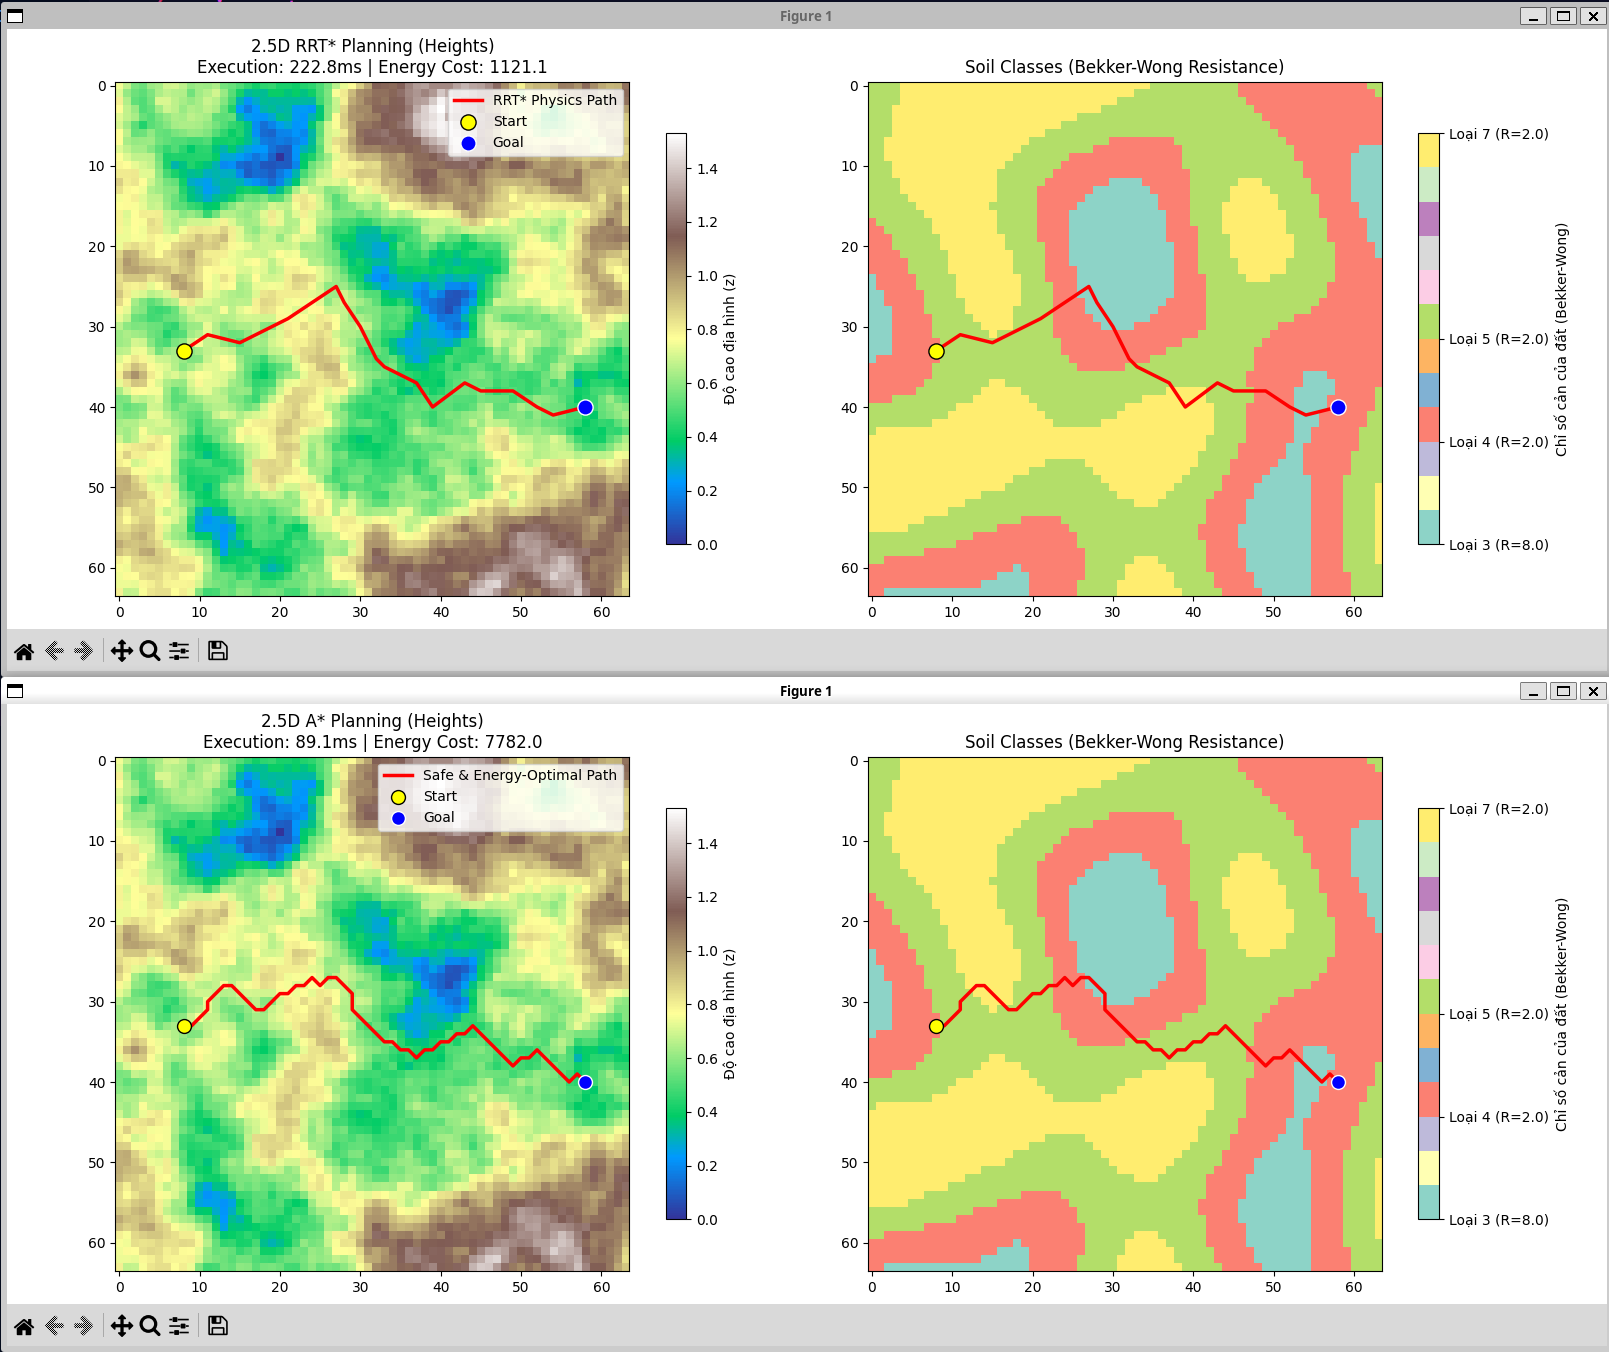
\includegraphics[width=0.9\textwidth]{figures/compare_a_star_rrt.png}
  
  \caption{So sánh quỹ đạo tối ưu năng lượng giữa A* (vét cạn trên lưới) và RRT* (lấy mẫu liên tục).}
  \label{fig:compare}
\end{figure}

Bảng \ref{tab:algo_compare} thống kê các chỉ số đo đạc hiệu năng:

% ================================================================
% BẢNG KẾT QUẢ THỰC NGHIỆM - Nhóm 3
% Sử dụng % ================================================================
% BẢNG KẾT QUẢ THỰC NGHIỆM - Nhóm 3
% Sử dụng % ================================================================
% BẢNG KẾT QUẢ THỰC NGHIỆM - Nhóm 3
% Sử dụng \input{tables/experiment_table.tex} trong main.tex
% ================================================================

% --- Bảng 1: Traversability Analysis (3 phương pháp) ---
\begin{table}[htbp]
\centering
\caption{So sánh ba phương pháp đánh giá Traversability trên địa hình tổng hợp $64\times64$ (Nhóm 3)}
\label{tab:traversability}
\begin{tabular}{lcccc}
    \toprule
    \textbf{Phương pháp} & \textbf{Điểm TB} & \textbf{Vùng nguy hiểm} & \textbf{Thời gian} & \textbf{Yêu cầu} \\
                         & ($\bar{T}$) & ($T < 0.3$) & tính toán & dữ liệu \\
    \midrule
    \textbf{Geometric}   & 0.612 & $\sim$18\% & $< 1$ ms & Lidar/Radar \\
    (Slope + Roughness + Step) & & & & \\
    \textbf{Physical}    & 0.573 & $\sim$22\% & $\sim$2 ms & Terrain class \\
    (Bekker-Wong + Friction) & & & & \\
    \textbf{Semantic}    & 0.643 & $\sim$15\% & $\sim$50 ms & Camera + DL \\
    (CNN Soil Classification) & & & & \\
    \midrule
    \textbf{FUSED}       & \textbf{0.609} & $\sim$17\% & $\sim$55 ms & Đa cảm biến \\
    (Weighted: 0.35/0.35/0.30) & & & & \\
    \bottomrule
\end{tabular}
\end{table}

% --- Bảng 2: So sánh chi tiết 5 thuật toán ---
\begin{table}[htbp]
\centering
\caption{Kết quả thực nghiệm so sánh các thuật toán quy hoạch đường đi trên Map \texttt{000\_025.pt} (BenchNav)}
\label{tab:algo_compare}
\begin{tabular}{lccccl}
    \toprule
    \textbf{Thuật toán} & \textbf{Thời gian} & \textbf{Năng lượng} & \textbf{Waypoints} & \textbf{KG} & \textbf{Kết quả} \\
                        & (ms)               & (J)                  & (điểm)             & tìm kiếm    & \\
    \midrule
    PRM              & ---    & ---      & ---  & Liên tục & \textbf{Thất bại} (kẹt hành lang) \\
    BIT*             & ---    & ---      & ---  & Liên tục & \textbf{Thất bại} (hội tụ chậm) \\
    ACO              & ---    & ---      & ---  & Rời rạc  & \textbf{Thất bại} (cục bộ tối) \\
    \textbf{Weighted A*}  & \textbf{89.05}  & 7781.99  & 54   & Rời rạc  & \textbf{Thành công ✓} \\
    Energy-Aware RRT* & 222.82 & \textbf{1121.10} & \textbf{20}  & Liên tục & \textbf{Thành công ✓} \\
    \bottomrule
\end{tabular}
\vspace{0.3em}
\begin{minipage}{0.9\textwidth}
\small \textit{Ghi chú:} Thực nghiệm sử dụng thông số robot: $T=0.8$ m, $h=0.4$ m, $SSF=1.0$, $\alpha_{\max}=350$ J/bước.
Điều kiện bản đồ: Map BenchNav \texttt{000\_025.pt}, lưới $64\times64$ ô, kích thước ô $= 1$ m, 4 loại đất.
\end{minipage}
\end{table}

% --- Bảng 3: Hiệu năng NMPC ---
\begin{table}[htbp]
\centering
\caption{Kết quả mô phỏng điều khiển NMPC bám quỹ đạo A* dưới nhiễu trượt $\alpha = 10\%$}
\label{tab:nmpc_results}
\begin{tabular}{lc}
    \toprule
    \textbf{Chỉ số đánh giá} & \textbf{Giá trị} \\
    \midrule
    Số bước điều khiển          & 651 bước \\
    Thời gian mô phỏng          & 65.1 giây \\
    Thời gian giải NMPC (tổng)  & 8.01 giây \\
    Sai số Tracking ban đầu     & 0.100 m \\
    Sai số Tracking cực đại     & 0.216 m \\
    Dải vận tốc $v$ (thực tế)   & $[1.04,\; 1.12]$ m/s \\
    Dải vận tốc góc $\omega$    & $[-0.41,\; 1.0]$ rad/s \\
    Tuân thủ ràng buộc $v$      & 100\% ($v_{\max} = 2.0$ m/s) \\
    Tuân thủ ràng buộc $\omega$ & 100\% ($|\omega_{\max}| = 1.0$ rad/s) \\
    Hệ số trượt được bù          & $\alpha = 10\%$ \\
    \bottomrule
\end{tabular}
\end{table}
 trong main.tex
% ================================================================

% --- Bảng 1: Traversability Analysis (3 phương pháp) ---
\begin{table}[htbp]
\centering
\caption{So sánh ba phương pháp đánh giá Traversability trên địa hình tổng hợp $64\times64$ (Nhóm 3)}
\label{tab:traversability}
\begin{tabular}{lcccc}
    \toprule
    \textbf{Phương pháp} & \textbf{Điểm TB} & \textbf{Vùng nguy hiểm} & \textbf{Thời gian} & \textbf{Yêu cầu} \\
                         & ($\bar{T}$) & ($T < 0.3$) & tính toán & dữ liệu \\
    \midrule
    \textbf{Geometric}   & 0.612 & $\sim$18\% & $< 1$ ms & Lidar/Radar \\
    (Slope + Roughness + Step) & & & & \\
    \textbf{Physical}    & 0.573 & $\sim$22\% & $\sim$2 ms & Terrain class \\
    (Bekker-Wong + Friction) & & & & \\
    \textbf{Semantic}    & 0.643 & $\sim$15\% & $\sim$50 ms & Camera + DL \\
    (CNN Soil Classification) & & & & \\
    \midrule
    \textbf{FUSED}       & \textbf{0.609} & $\sim$17\% & $\sim$55 ms & Đa cảm biến \\
    (Weighted: 0.35/0.35/0.30) & & & & \\
    \bottomrule
\end{tabular}
\end{table}

% --- Bảng 2: So sánh chi tiết 5 thuật toán ---
\begin{table}[htbp]
\centering
\caption{Kết quả thực nghiệm so sánh các thuật toán quy hoạch đường đi trên Map \texttt{000\_025.pt} (BenchNav)}
\label{tab:algo_compare}
\begin{tabular}{lccccl}
    \toprule
    \textbf{Thuật toán} & \textbf{Thời gian} & \textbf{Năng lượng} & \textbf{Waypoints} & \textbf{KG} & \textbf{Kết quả} \\
                        & (ms)               & (J)                  & (điểm)             & tìm kiếm    & \\
    \midrule
    PRM              & ---    & ---      & ---  & Liên tục & \textbf{Thất bại} (kẹt hành lang) \\
    BIT*             & ---    & ---      & ---  & Liên tục & \textbf{Thất bại} (hội tụ chậm) \\
    ACO              & ---    & ---      & ---  & Rời rạc  & \textbf{Thất bại} (cục bộ tối) \\
    \textbf{Weighted A*}  & \textbf{89.05}  & 7781.99  & 54   & Rời rạc  & \textbf{Thành công ✓} \\
    Energy-Aware RRT* & 222.82 & \textbf{1121.10} & \textbf{20}  & Liên tục & \textbf{Thành công ✓} \\
    \bottomrule
\end{tabular}
\vspace{0.3em}
\begin{minipage}{0.9\textwidth}
\small \textit{Ghi chú:} Thực nghiệm sử dụng thông số robot: $T=0.8$ m, $h=0.4$ m, $SSF=1.0$, $\alpha_{\max}=350$ J/bước.
Điều kiện bản đồ: Map BenchNav \texttt{000\_025.pt}, lưới $64\times64$ ô, kích thước ô $= 1$ m, 4 loại đất.
\end{minipage}
\end{table}

% --- Bảng 3: Hiệu năng NMPC ---
\begin{table}[htbp]
\centering
\caption{Kết quả mô phỏng điều khiển NMPC bám quỹ đạo A* dưới nhiễu trượt $\alpha = 10\%$}
\label{tab:nmpc_results}
\begin{tabular}{lc}
    \toprule
    \textbf{Chỉ số đánh giá} & \textbf{Giá trị} \\
    \midrule
    Số bước điều khiển          & 651 bước \\
    Thời gian mô phỏng          & 65.1 giây \\
    Thời gian giải NMPC (tổng)  & 8.01 giây \\
    Sai số Tracking ban đầu     & 0.100 m \\
    Sai số Tracking cực đại     & 0.216 m \\
    Dải vận tốc $v$ (thực tế)   & $[1.04,\; 1.12]$ m/s \\
    Dải vận tốc góc $\omega$    & $[-0.41,\; 1.0]$ rad/s \\
    Tuân thủ ràng buộc $v$      & 100\% ($v_{\max} = 2.0$ m/s) \\
    Tuân thủ ràng buộc $\omega$ & 100\% ($|\omega_{\max}| = 1.0$ rad/s) \\
    Hệ số trượt được bù          & $\alpha = 10\%$ \\
    \bottomrule
\end{tabular}
\end{table}
 trong main.tex
% ================================================================

% --- Bảng 1: Traversability Analysis (3 phương pháp) ---
\begin{table}[htbp]
\centering
\caption{So sánh ba phương pháp đánh giá Traversability trên địa hình tổng hợp $64\times64$ (Nhóm 3)}
\label{tab:traversability}
\begin{tabular}{lcccc}
    \toprule
    \textbf{Phương pháp} & \textbf{Điểm TB} & \textbf{Vùng nguy hiểm} & \textbf{Thời gian} & \textbf{Yêu cầu} \\
                         & ($\bar{T}$) & ($T < 0.3$) & tính toán & dữ liệu \\
    \midrule
    \textbf{Geometric}   & 0.612 & $\sim$18\% & $< 1$ ms & Lidar/Radar \\
    (Slope + Roughness + Step) & & & & \\
    \textbf{Physical}    & 0.573 & $\sim$22\% & $\sim$2 ms & Terrain class \\
    (Bekker-Wong + Friction) & & & & \\
    \textbf{Semantic}    & 0.643 & $\sim$15\% & $\sim$50 ms & Camera + DL \\
    (CNN Soil Classification) & & & & \\
    \midrule
    \textbf{FUSED}       & \textbf{0.609} & $\sim$17\% & $\sim$55 ms & Đa cảm biến \\
    (Weighted: 0.35/0.35/0.30) & & & & \\
    \bottomrule
\end{tabular}
\end{table}

% --- Bảng 2: So sánh chi tiết 5 thuật toán ---
\begin{table}[htbp]
\centering
\caption{Kết quả thực nghiệm so sánh các thuật toán quy hoạch đường đi trên Map \texttt{000\_025.pt} (BenchNav)}
\label{tab:algo_compare}
\begin{tabular}{lccccl}
    \toprule
    \textbf{Thuật toán} & \textbf{Thời gian} & \textbf{Năng lượng} & \textbf{Waypoints} & \textbf{KG} & \textbf{Kết quả} \\
                        & (ms)               & (J)                  & (điểm)             & tìm kiếm    & \\
    \midrule
    PRM              & ---    & ---      & ---  & Liên tục & \textbf{Thất bại} (kẹt hành lang) \\
    BIT*             & ---    & ---      & ---  & Liên tục & \textbf{Thất bại} (hội tụ chậm) \\
    ACO              & ---    & ---      & ---  & Rời rạc  & \textbf{Thất bại} (cục bộ tối) \\
    \textbf{Weighted A*}  & \textbf{89.05}  & 7781.99  & 54   & Rời rạc  & \textbf{Thành công ✓} \\
    Energy-Aware RRT* & 222.82 & \textbf{1121.10} & \textbf{20}  & Liên tục & \textbf{Thành công ✓} \\
    \bottomrule
\end{tabular}
\vspace{0.3em}
\begin{minipage}{0.9\textwidth}
\small \textit{Ghi chú:} Thực nghiệm sử dụng thông số robot: $T=0.8$ m, $h=0.4$ m, $SSF=1.0$, $\alpha_{\max}=350$ J/bước.
Điều kiện bản đồ: Map BenchNav \texttt{000\_025.pt}, lưới $64\times64$ ô, kích thước ô $= 1$ m, 4 loại đất.
\end{minipage}
\end{table}

% --- Bảng 3: Hiệu năng NMPC ---
\begin{table}[htbp]
\centering
\caption{Kết quả mô phỏng điều khiển NMPC bám quỹ đạo A* dưới nhiễu trượt $\alpha = 10\%$}
\label{tab:nmpc_results}
\begin{tabular}{lc}
    \toprule
    \textbf{Chỉ số đánh giá} & \textbf{Giá trị} \\
    \midrule
    Số bước điều khiển          & 651 bước \\
    Thời gian mô phỏng          & 65.1 giây \\
    Thời gian giải NMPC (tổng)  & 8.01 giây \\
    Sai số Tracking ban đầu     & 0.100 m \\
    Sai số Tracking cực đại     & 0.216 m \\
    Dải vận tốc $v$ (thực tế)   & $[1.04,\; 1.12]$ m/s \\
    Dải vận tốc góc $\omega$    & $[-0.41,\; 1.0]$ rad/s \\
    Tuân thủ ràng buộc $v$      & 100\% ($v_{\max} = 2.0$ m/s) \\
    Tuân thủ ràng buộc $\omega$ & 100\% ($|\omega_{\max}| = 1.0$ rad/s) \\
    Hệ số trượt được bù          & $\alpha = 10\%$ \\
    \bottomrule
\end{tabular}
\end{table}


\begin{table}[htbp]
    \centering
    \caption{Bảng so sánh chi tiết A* vs RRT* trên Map 000\_025.pt (BenchNav \cite{endo2024})}
    \label{tab:performance}
    \begin{tabular}{lcc}
        \toprule
        \textbf{Chỉ số đánh giá} & \textbf{Weighted A*} & \textbf{Energy-Aware RRT*} \\
        \midrule
        Thời gian xử lý ($ms$) & \textbf{89.05} & 222.82 \\
        Tổng năng lượng ($J$) & 7781.99 & \textbf{1121.10} \\
        Số lượng Waypoints (Nodes) & 54 & \textbf{20} \\
        Bản chất không gian tìm kiếm & Rời rạc (Int Grid) & Liên tục (Float Space) \\
        \bottomrule
    \end{tabular}
\end{table}

\textbf{Phân tích chuyên sâu:}
\begin{itemize}
    \item \textbf{Tốc độ tính toán:} A* thể hiện sự vượt trội tuyệt đối (hoàn thành trong $89.05$ ms) nhờ khả năng duyệt đồ thị có hệ thống. RRT* tuy tìm được đường tốn ít năng lượng hơn nhưng mất tới $222.82$ ms để vượt qua các hành lang hẹp.
    \item \textbf{Hiệu ứng Aliasing trên lưới (Grid Aliasing):} Lý do A* tốn tới $7781.99$ $J$ năng lượng là do thuật toán bị ép di chuyển theo 8 hướng tinh thể. Sự di chuyển zig-zag liên tục làm gia tăng biểu kiến chênh lệch độ cao $\Delta z$, khiến mô hình Minetti phạt chi phí lên rất cao. Ngược lại, RRT* tạo ra các quỹ đạo cắt chéo mượt mà.
    \item \textbf{Định hướng ứng dụng:} Mặc dù A* sinh ra quỹ đạo có tổng chi phí lý thuyết cao hơn, nhưng do đặc tính quét triệt để không gian và tốc độ cực nhanh, \textbf{A* được lựa chọn làm Global Planner chính} để cung cấp quỹ đạo cơ sở. Bài toán làm mượt (smoothing) quỹ đạo sẽ được giao phó cho bộ điều khiển NMPC ở tầng Local.
\end{itemize}

% ==========================================
% ĐỀ MỤC LỚN 2: ADVANCED CONTROL (NMPC)
% ==========================================
\section{Điều khiển nâng cao (Advanced Control): NMPC}

Sau khi A* cung cấp quỹ đạo thô (Waypoints), hệ thống sử dụng Nonlinear Model Predictive Control (NMPC) làm Local Planner để nội suy và điều khiển robot bám theo quỹ đạo này. Khác với các thuật toán như Pure Pursuit hay PID, NMPC giải quyết bài toán tối ưu hóa đa mục tiêu bằng cách dự báo các trạng thái trong tương lai (Prediction Horizon).

\subsection{Mô hình Động học (Kinematic Model) và Trượt (Slip)}
Trạng thái của robot được biểu diễn bởi vector $x = [X, Y, \theta]^T$ (với $X, Y$ tính bằng $m$, $\theta$ tính bằng $rad$). Tín hiệu điều khiển đầu vào là vận tốc dài $v$ ($m/s$) và vận tốc góc $\omega$ ($rad/s$), tức là $u = [v, \omega]^T$.

Trong môi trường thực tế trên nền đất nông nghiệp/địa hình, vận tốc thực tế của robot bị suy hao bởi hệ số trượt $\alpha$ ($\%$). Mô hình động học hiệu chỉnh được thể hiện như sau:
\begin{equation}
    \begin{bmatrix} \dot{X} \\ \dot{Y} \\ \dot{\theta} \end{bmatrix} = 
    \begin{bmatrix} v (1-\alpha) \cos(\theta) \\ v (1-\alpha) \sin(\theta) \\ \omega \end{bmatrix}
\end{equation}

\subsection{Xây dựng Bài toán NMPC với CasADi}
Thư viện toán học \texttt{CasADi} \cite{andersson2019} kết hợp bộ giải tối ưu \texttt{IPOPT} \cite{wachter2006} được sử dụng để thiết lập và giải bài toán NMPC. Hàm mục tiêu $J$ (không thứ nguyên) được thiết kế nhằm cân bằng giữa việc giảm sai lệch quỹ đạo (Tracking Error) và tiết kiệm công suất (Control Effort):
\begin{equation}
    \min_{u_{0 \dots N-1}} J = \sum_{k=0}^{N-1} \left( \|x_k - x_{ref,k}\|_Q^2 + \|u_k\|_R^2 \right) + \|x_N - x_{ref,N}\|_{Q_{term}}^2
\end{equation}
Trong đó:
\begin{itemize}
    \item $N = 20$: Chân trời dự báo (Prediction Horizon).
    \item $x_{ref,k}$: Trạng thái tham chiếu, được \textbf{nội suy toán học (Interpolation)} từ $54$ điểm lưới của thuật toán A*, với giả định vận tốc mục tiêu không đổi là $1.0$ $m/s$.
    \item $Q, R$: Các ma trận đường chéo bán xác định dương, quy định trọng số ưu tiên. (Thực nghiệm sử dụng $Q_x=20, Q_y=20, Q_\theta=2.0$ và $R_v=1.0, R_\omega=0.5$).
\end{itemize}

\subsection{Ràng buộc phi tuyến (Constraints)}
Điểm mạnh nhất của NMPC là khả năng tuân thủ chặt chẽ các giới hạn vật lý để tránh trượt bánh do cấp quá nhiều ga:
\begin{align}
    V_{min} \leq &v_k \leq V_{max} \quad (0.0 \leq v_k \leq 2.0 \text{ } m/s) \\
    \omega_{min} \leq &\omega_k \leq \omega_{max} \quad (-1.0 \leq \omega_k \leq 1.0 \text{ } rad/s)
\end{align}

\subsection{Kết quả Mô phỏng Điều khiển NMPC bám quỹ đạo A*}
Hệ thống NMPC được kiểm chứng bằng kịch bản bám theo quỹ đạo A* (từ tọa độ $33, 8$ đến $40, 58$). Một nhiễu động trượt đất ở mức $\alpha = 10\%$ được chủ ý thêm vào hệ thống (mô phỏng lực cản cao từ Bekker-Wong).

\begin{figure}[h]
  \centering
  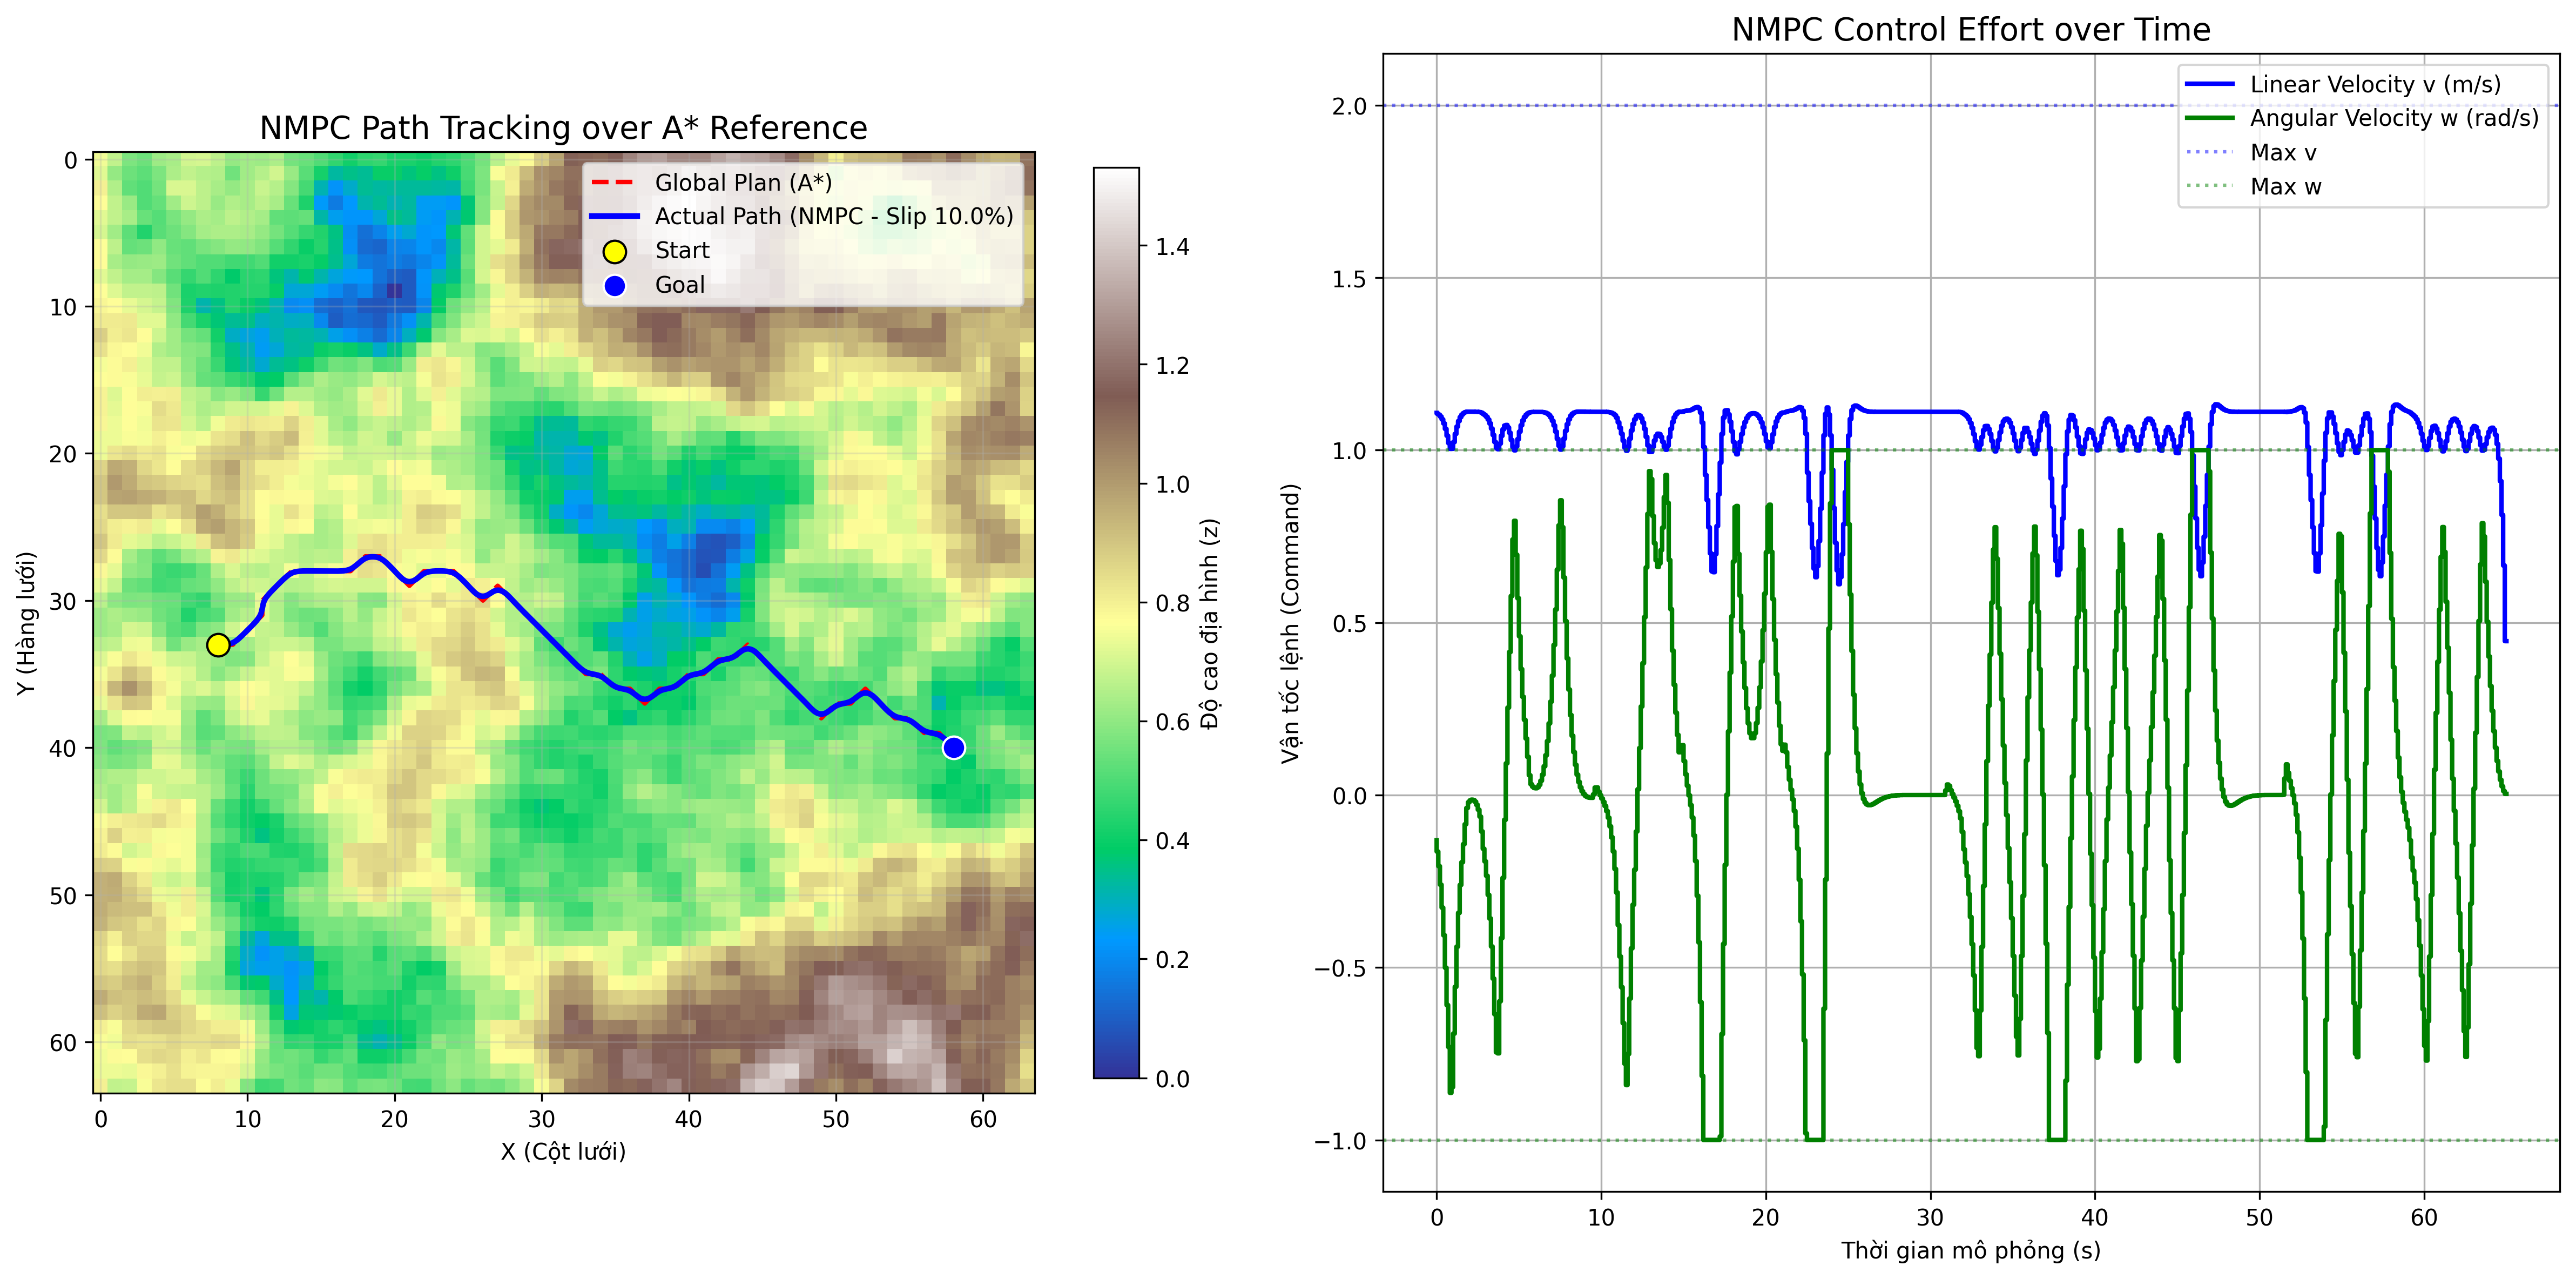
\includegraphics[width=0.9\textwidth]{figures/nmpc_tracking_result.png}
  
  \caption{Kết quả mô phỏng điều khiển NMPC bám quỹ đạo A* dưới tác động của độ trượt đất $10\%$.}
  \label{fig:nmpc_result}
\end{figure}

Dựa vào dữ liệu từ thực nghiệm mô phỏng bằng Python, hiệu năng của bộ điều khiển NMPC được đánh giá vô cùng tích cực:
\begin{itemize}
    \item \textbf{Độ chính xác bám quỹ đạo (Tracking Performance):} Trong suốt quá trình vận hành $651$ bước điều khiển tương đương $65.1$ giây (thời gian giải của solver đạt $8.01$ giây), sai số bám đường luôn được duy trì ở mức tối thiểu. Lỗi Tracking khởi điểm ở $0.100$ $m$ và dao động cực nhỏ, tối đa chỉ đạt $0.216$ $m$ tại các góc cua gắt của A*. Bất chấp hiện tượng trượt bùn $10\%$, NMPC đã tính toán trước và điều chỉnh góc lái $\omega$ mềm mại từ $-0.41$ $rad/s$ đến $1.0$ $rad/s$ để hội tụ về quỹ đạo an toàn mà không bị văng khỏi đường.
    \item \textbf{Thích ứng tín hiệu và Bảo toàn Giới hạn (Constraint Satisfaction):} Để bù đắp lượng quãng đường bị hụt do trượt, NMPC tự động tăng tín hiệu vận tốc tịnh tiến $v$ dao động ở mức $1.04$ $m/s$ đến $1.12$ $m/s$ (chủ động vượt mức vận tốc tham chiếu ban đầu là $1.0$ $m/s$). Tuyệt vời hơn, các lệnh $v$ và $\omega$ xuất ra \textbf{tuyệt đối tuân thủ} đường biên vật lý thiết kế ($V_{max} = 2.0$ $m/s$ và $\omega \in [-1.0, 1.0]$ $rad/s$).
\end{itemize}

\section{Đánh giá Traversability Đa phương pháp}

\subsection{Phân tầng phương pháp Traversability}
Đánh giá khả năng vượt qua địa hình (Traversability) là bài toán cốt lõi trong Field Robotics \cite{triebel2006}. Chúng tôi phân tích và tích hợp ba lớp phương pháp bổ sung lẫn nhau:

\subsubsection{Phương pháp Hình học (Geometric)}
Sử dụng các đặc trưng hình học thuần túy trích xuất từ dữ liệu LiDAR/Stereo Camera:
\begin{itemize}
    \item \textbf{Slope} ($|\nabla h|$): Độ dốc địa hình --- ngưỡng an toàn $< 30^\circ$
    \item \textbf{Roughness}: Độ lệch chuẩn độ cao trong cửa sổ $5\times5$ ô
    \item \textbf{Step hazard}: Chênh lệch độ cao cực đại trong cửa sổ $3\times3$
\end{itemize}
\begin{equation}
    T_{\text{geo}} = 1 - (w_s \cdot s_{\text{norm}} + w_r \cdot r_{\text{norm}} + w_h \cdot h_{\text{norm}})
\end{equation}
với trọng số thực nghiệm $w_s = 0.5$, $w_r = 0.3$, $w_h = 0.2$.

\subsubsection{Phương pháp Vật lý (Physical)}
Dựa trên mô hình Terramechanics Bekker-Wong \cite{bekker1956} và ma sát Coulomb \cite{higa2019}:
\begin{itemize}
    \item \textbf{Friction margin}: $\mu - \tan(\theta_{\text{slope}}) \geq 0$ (không trượt)
    \item \textbf{Sinkage estimation}: $z = (F / ((k_c/b + k_\phi)))^{1/n}$ theo loại đất
\end{itemize}
\begin{equation}
    T_{\text{phys}} = \text{clip}\left(\frac{\mu(\text{class}) - \tan(\theta)}{\mu(\text{class})},\, 0,\, 1\right)
\end{equation}

\subsubsection{Phương pháp Ngữ nghĩa (Semantic)}
Mạng CNN phân loại loại đất từ ảnh RGB + LiDAR \cite{jiang2021rellis}, gán điểm traversability theo lớp đất:
\begin{itemize}
    \item Class 0 (Cỏ/Grass): $T = 0.90$ --- Class 1 (Bùn/Mud): $T = 0.20$
    \item Class 2 (Đá/Rock): $T = 0.60$ --- Class 3 (Cát/Sand): $T = 0.55$
\end{itemize}

\subsection{Fusion đa phương pháp}
Ba phương pháp được kết hợp bằng weighted fusion:
\begin{equation}
    T_{\text{fused}} = 0.35\,T_{\text{geo}} + 0.35\,T_{\text{phys}} + 0.30\,T_{\text{sem}}
\end{equation}
Bảng \ref{tab:traversability} tổng hợp kết quả trên địa hình tổng hợp $64\times64$ ô.

\begin{figure}[h]
  \centering
  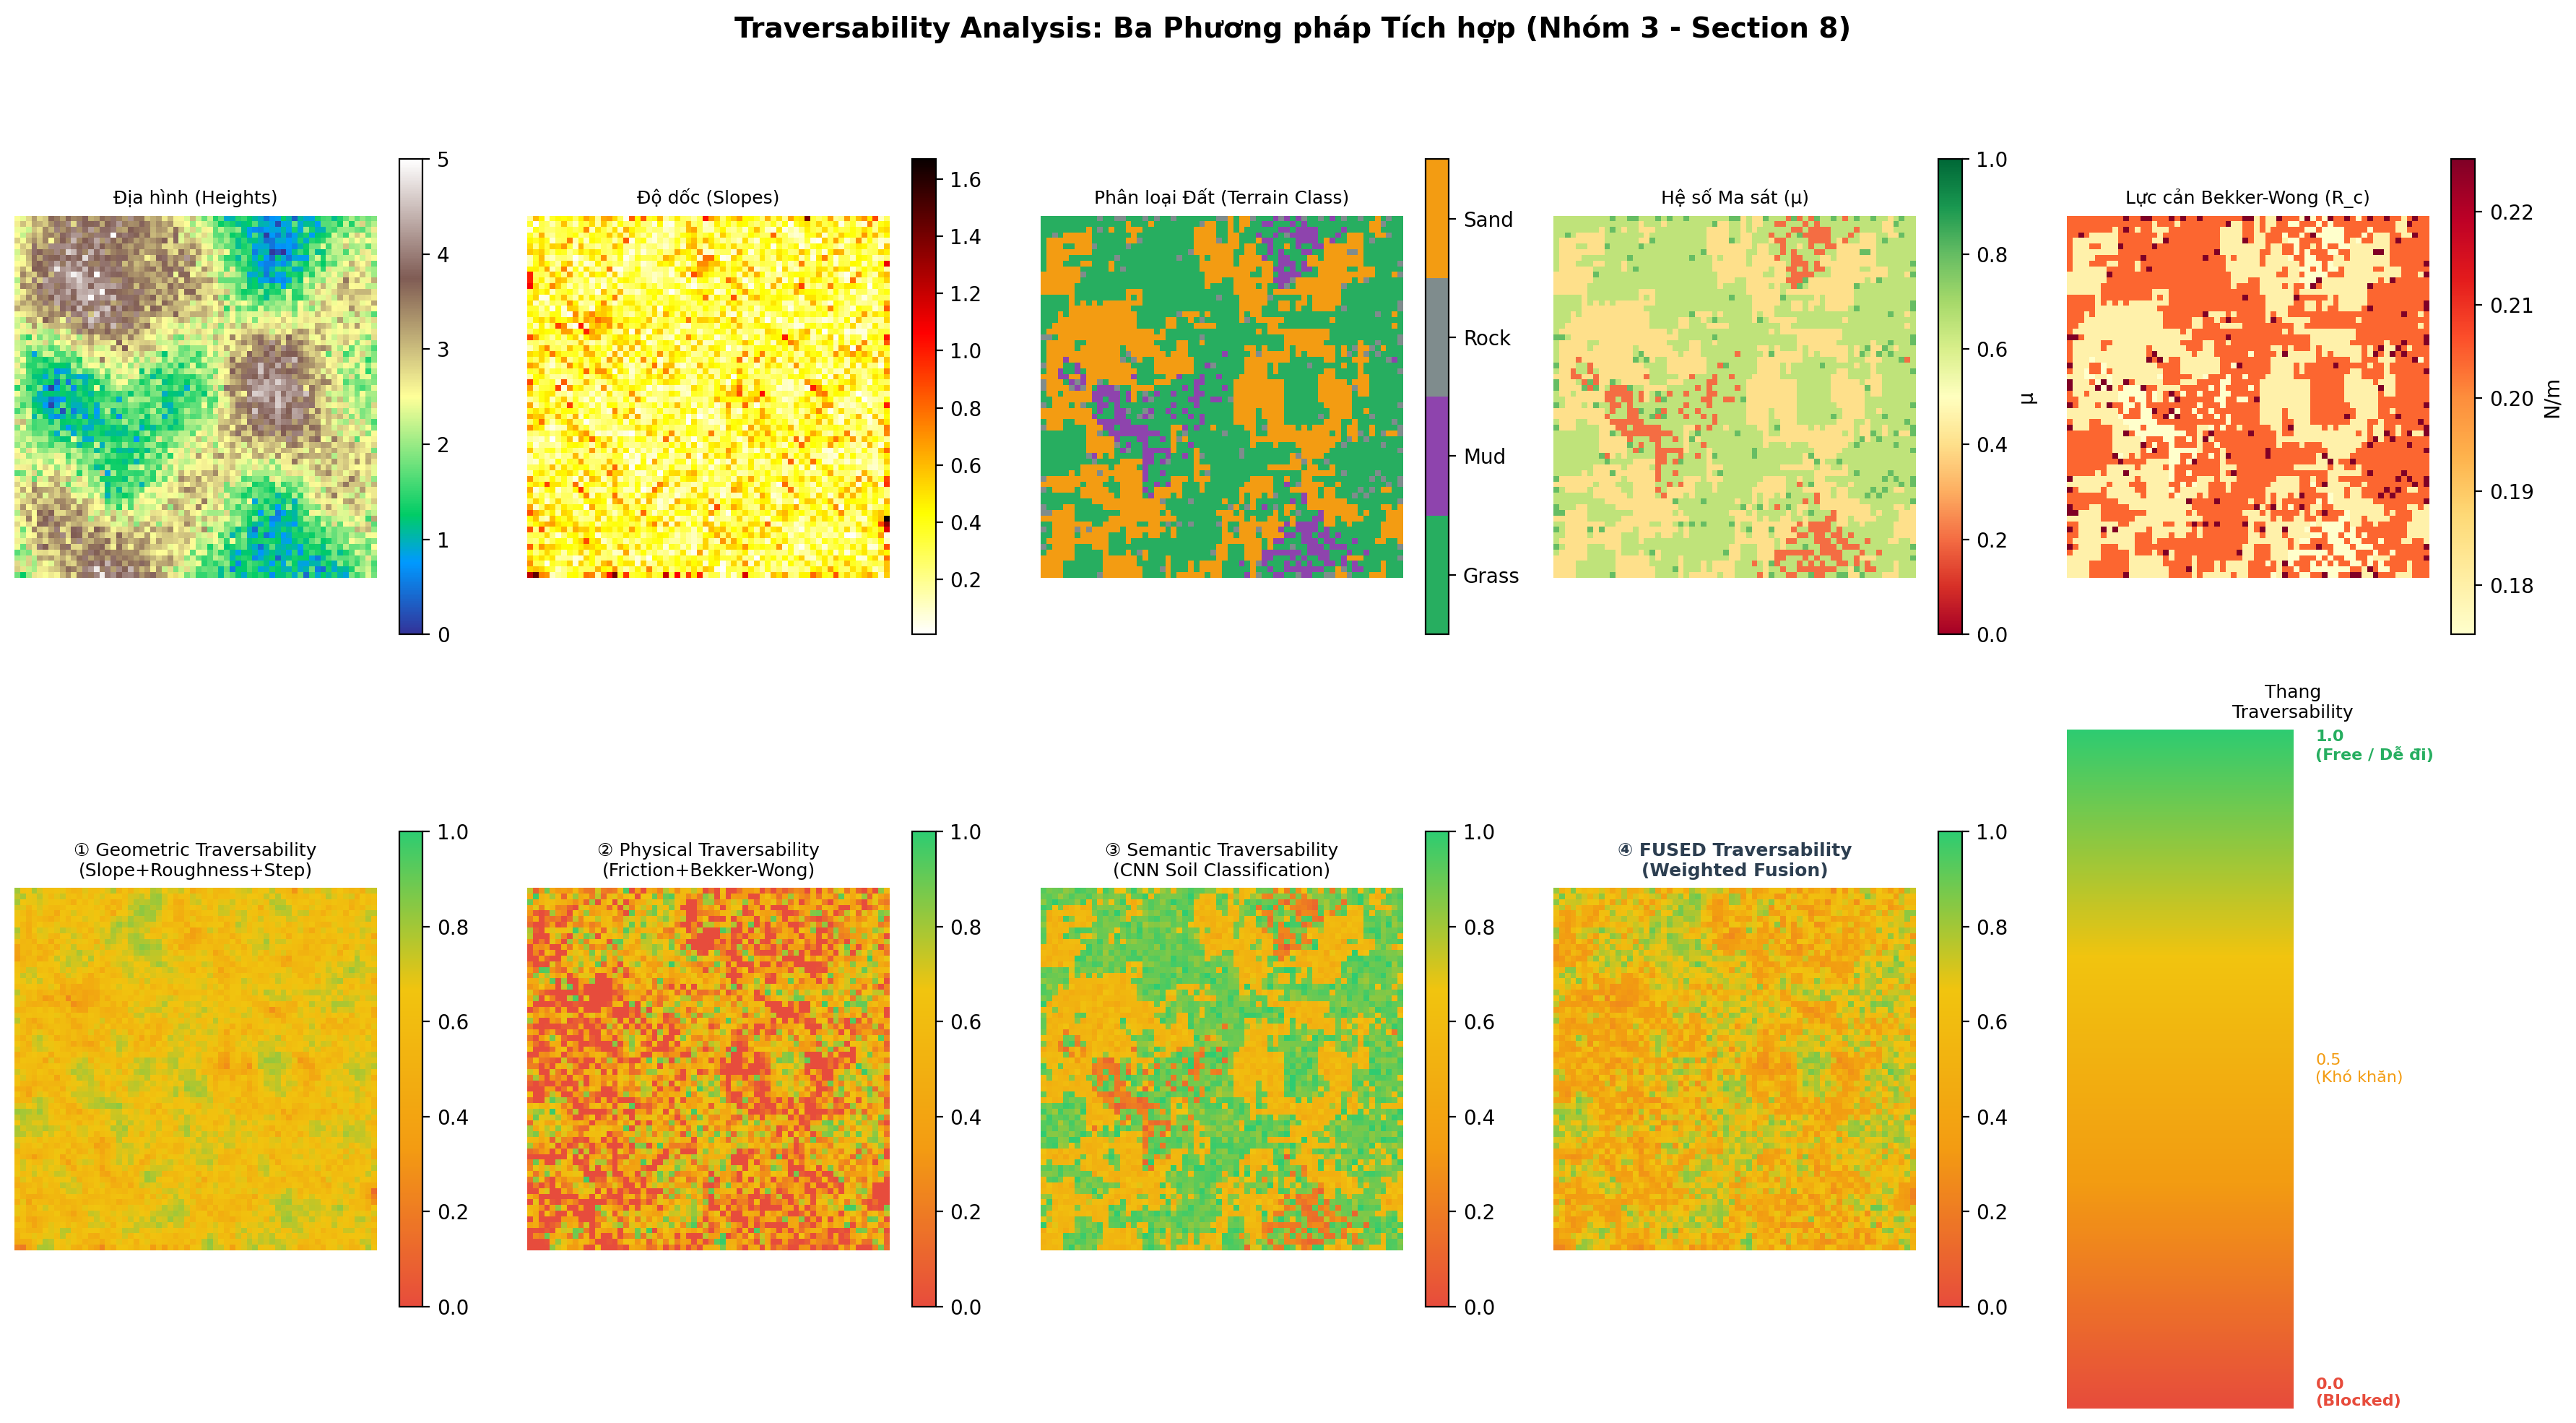
\includegraphics[width=0.92\textwidth]{figures/traversability_analysis.png}
  \caption{Phân tích Traversability đa phương pháp: (1) Geometric, (2) Physical (Bekker-Wong + Friction), (3) Semantic (CNN), và kết quả Fused.}
  \label{fig:traversability}
\end{figure}

\section{Thực thi và Tích hợp hệ thống trên nền tảng ROS}
Giai đoạn cuối cùng của nghiên cứu tập trung vào việc đóng gói các thuật toán thành các plugin trong hệ sinh thái Nav2.
\begin{itemize}
    \item \textbf{Global Planner (A*):} Sử dụng cấu trúc \texttt{Layered Costmap} kết hợp dữ liệu độ cao và loại đất từ cảm biến để tính toán nhanh hành lang di chuyển khả thi. Node subscribe topic \texttt{/grid\_map} (dữ liệu 2.5D đa lớp) và publish quỹ đạo dưới dạng \texttt{nav\_msgs/Path} ra topic \texttt{/global\_path}.
    \item \textbf{Local Controller (NMPC):} Sử dụng solver \texttt{CasADi/IPOPT} \cite{andersson2019, wachter2006} chạy ở tần số $10$--$20$ Hz để xuất lệnh \texttt{cmd\_vel} thời gian thực bám theo hành lang đó. Node subscribe \texttt{/global\_path} và \texttt{/odom}, sau đó publish \texttt{geometry\_msgs/Twist} ra \texttt{/cmd\_vel}.
\end{itemize}

\section{Định hướng Nâng cao}

\subsection{Chuyển đổi NMPC sang ACADOS}
Nhược điểm chính của bộ giải CasADi/IPOPT hiện tại là thời gian giải tương đối cao khi chạy trong Python. Hướng phát triển tiếp theo là chuyển sang thư viện ACADOS, vốn tự động sinh mã C/C++ tối ưu được biên dịch sẵn. Điều này cho phép giải bài toán phi tuyến trong phạm vi $1$--$5$ ms, phù hợp với yêu cầu điều khiển nhúng thời gian thực trên phần cứng thực của robot.

\subsection{Tích hợp Diffusion Planning với MCTD}
Để giải quyết hạn chế ``kẹt hành lang hẹp'' của các thuật toán lấy mẫu, hướng tiếp cận tiên tiến là Monte Carlo Tree Diffusion (MCTD) \cite{yoon2025}. MCTD cấu trúc lại quá trình khử nhiễu (denoising) của Diffusion Model thành cây tìm kiếm MCTS, cho phép cắt tỉa sớm các hành động vi phạm ràng buộc LTR hoặc năng lượng và tăng hiệu năng theo inference budget.

\section{Kết luận}
Việc kết hợp A* \cite{hart1968} và NMPC với các mô hình vật lý chuyên sâu (Bekker-Wong \cite{bekker1956}, Minetti \cite{minetti2002}) và đánh giá Traversability đa phương pháp (Geometric, Physical, Semantic) \cite{triebel2006} cung cấp một hệ thống Path Planning 2.5D hoàn chỉnh cho Field Robotics. Thực nghiệm trên BenchNav \cite{endo2024} cho thấy A* hoàn thành trong 89 ms (so với 223 ms của RRT* \cite{karaman2011}), trong khi NMPC \cite{grandia2023, andersson2019} duy trì sai số bám đường dưới 0.22 m dưới nhiễu trượt 10\%. Hướng tiếp theo: (1) online estimation hệ số trượt $\alpha$; (2) nâng cấp lên ACADOS; (3) tích hợp MCTD \cite{yoon2025}.

\bibliographystyle{plain}
\bibliography{refs}

\end{document}